\documentclass[11pt,a4paper]{article}

% ---------- Layout & fonts ----------
\usepackage[a4paper,margin=2.6cm]{geometry}
\usepackage{libertinus}
\usepackage[T1]{fontenc}
\usepackage{microtype}
\usepackage{xcolor}
\usepackage{tikz}
\usetikzlibrary{arrows.meta}
\usepackage{parskip}

% ---------- Title block ----------
\usepackage{titling}
\setlength{\droptitle}{-2.2cm}
\pretitle{%
  \begin{center}
  \rule{\linewidth}{0.8pt}\vspace{7pt}\par
  \LARGE\scshape}
\posttitle{\par\vspace{5pt}\rule{\linewidth}{0.4pt}\end{center}}
\preauthor{\begin{center}\normalsize\color{black!60}}
\postauthor{\end{center}}
\predate{}\postdate{}

% ---------- Section headings ----------
\usepackage{titlesec}
\titleformat{\section}
  {\normalfont\large\scshape}{\thesection}{0.8em}{}
  [\vspace{-0.7em}\color{black!35}\rule{\linewidth}{0.4pt}]
\titlespacing*{\section}{0pt}{2.4ex plus 1ex minus .2ex}{1.4ex plus .2ex}

\titleformat{\subsection}
  {\normalfont\normalsize\bfseries}{\thesubsection}{0.8em}{}
\titlespacing*{\subsection}{0pt}{2ex plus .8ex minus .2ex}{0.8ex plus .2ex}

% ---------- Math ----------
\usepackage{amsmath,amssymb,amsthm}

% ---------- Floats & boxes ----------
\usepackage{graphicx}
\usepackage[font=small,labelfont=bf]{caption}
\usepackage{tcolorbox}
\usepackage[colorlinks=true,allcolors=black!70!blue]{hyperref}

% ---------- Theorem environments ----------
\theoremstyle{plain}
\newtheorem{lemma}{Lemma}
\newtheorem{proposition}{Proposition}
\theoremstyle{remark}
\newtheorem*{remark}{Remark}

\title{Some Off Square}
\author{Pulvsama}
\date{}

\begin{document}

\maketitle

\section*{Problem}

\begin{figure}[!ht]
    \centering
    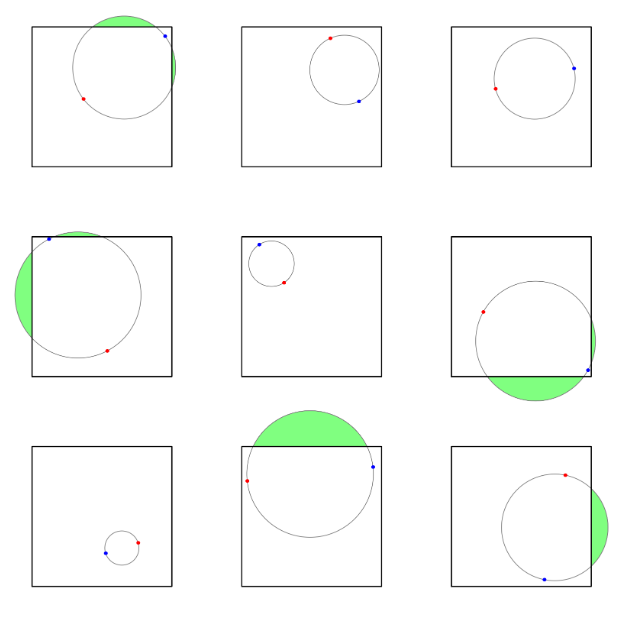
\includegraphics[width=0.6\textwidth]{Examples.png}
    \caption{Description of the figure}
\end{figure}

\begin{tcolorbox}[colback=black!3,colframe=black!25,boxrule=0.4pt,arc=2pt]
A circle is randomly generated by sampling two points uniformly and independently from the interior of a square and using these points to determine its diameter. What is the probability that the circle has a part of it that is off the square? 

\textbf{Give your answer in exact terms}.
\end{tcolorbox}

\newpage

\section*{Solution}

\subsection*{Setup and notations}

Before doing anything, let me first define the setup we are going to work with. Nothing is said about dimensions and it doesn't really matter in this puzzle, the square might be of side legnth $a$ but we are going to arbitrarily set it to 2.
\\
Set Cartesian coordinates with origin at the centre of the square and axes parallel to its sides, so that the square is
\[
    S = [-1,1]^2 .
\]
\begin{figure}[!ht]
\centering
\begin{tikzpicture}[scale=2, >={Stealth[length=5pt]}]
    \draw[->, black!55] (-1.5,0) -- (1.5,0) node[right, black] {$x$};
    \draw[->, black!55] (0,-1.5) -- (0,1.5) node[above, black] {$y$};

    \draw[thick] (-1,-1) rectangle (1,1);

    \draw (1,0.04) -- (1,-0.04) node[below right, font=\small] {$1$};
    \draw (-1,0.04) -- (-1,-0.04) node[below left, font=\small] {$-1$};
    \draw (0.04, 1) -- (-0.04, 1) node[above right, font=\small] {$1$};
    \draw (0.04, -1) -- (-0.04, -1) node[below right, font=\small] {$-1$};

    \fill (0,0) circle (0.025) node[below left, font=\small] {$O$};

    \fill[red] (0.5, 0.3) circle (0.025) node[above right, font=\small] {$(x_1, y_1)$};
    \fill[blue] (-0.1, -0.4) circle (0.025) node[below left, font=\small] {$(x_2, y_2)$};

    \draw[very thin] (0.2, -0.05) circle ({sqrt(0.6^2 + 0.7^2)/2});
\end{tikzpicture}
\caption{The square $S=[-1,1]^2$.}
\end{figure}

That way, we can define our two points $p_1=(x_1, y_1)$ and $p_2 = (x_2, y_2)$  as coordinates. 
\\
A random point in the square is thus $(X, Y) \sim \mathcal{U}(S)$ ($X$ and $Y$ are independent)

\subsection*{Reformulating the problem}

Fix two points $p_1 = (x_1,y_1)$ and $p_2 = (x_2,y_2)$ in $S$. They span a diameter of a circle $\mathcal{C}$ with centre and radius
\[
    O_C = \frac{p_1 + p_2}{2},
    \qquad
    r = \frac{\lVert p_1 - p_2 \rVert}{2},
\]
so that
\[
    \mathcal{C} = \left\{\, O_C + r\begin{pmatrix}\cos\theta \\ \sin\theta \end{pmatrix}
    \;\middle|\; \theta \in [0, 2\pi) \,\right\}.
\]
The circle lies inside the square precisely when every point of $\mathcal{C}$ does, and we now turn this into a condition on $x_1, x_2, y_1, y_2$ alone.

Let $p_\theta \in \mathcal{C}$, i.e. $p_\theta = O_C + r\begin{pmatrix}\cos\theta\\ \sin\theta\end{pmatrix}$ for some $\theta \in [0, 2\pi)$.

Obviously if the circle lies inside the square, $p_\theta$ necessarily is inside the square
\begin{align*}
    p_\theta \in S
    &\iff
    \frac{p_1 + p_2}{2} + r \begin{pmatrix}\cos\theta \\ \sin\theta \end{pmatrix} \in S
    \\
    &\iff
    \begin{cases}
        \dfrac{x_1 + x_2}{2} + r \cos \theta \in [-1, 1] \\[6pt]
        \dfrac{y_1 + y_2}{2} + r \sin \theta \in [-1, 1]
    \end{cases}
\end{align*}

Since it's supposed to hold for all $\theta \in [0, 2\pi)$, it is necessarily true for $\theta = 0$, $\theta = \pi$, $\theta = \frac{\pi}{2}$ and $\theta = \frac{3\pi}{2}$

This gives us 4 conditions on $(x_1, x_2, y_1, y_2)$ to work on:

\begin{align*}
    \begin{cases}
        \dfrac{x_1 + x_2}{2} + r  \leq 1 \\[6pt]
        \dfrac{y_1 + y_2}{2} + r  \leq 1 \\[6pt]
        \dfrac{x_1 + x_2}{2} - r  \geq -1 \\[6pt]
        \dfrac{y_1 + y_2}{2} - r  \geq -1
    \end{cases}
    & \iff
    \begin{cases}
        r - 1 \leq \dfrac{x_1 + x_2}{2} \leq 1 - r \\[6pt]
        r - 1 \leq \dfrac{y_1 + y_2}{2} \leq 1 - r \\[6pt]
    \end{cases}
    \\[20pt]
    & \iff
    \begin{cases}
        |x_1 + x_2| \leq 2(1-r) \\
        |y_1 + y_2| \leq 2(1-r)
    \end{cases}
\end{align*}
Now how do we make sure that these are sufficient conditons for the circle to lie in the square ?

Conversely, assume that
\[
    |x_1 + x_2| \leq 2(1-r)
    \qquad \text{and} \qquad
    |y_1 + y_2| \leq 2(1-r).
\]
Let $\theta \in [0, 2\pi)$ be arbitrary. By the triangle inequality, and since $|\cos\theta| \leq 1$,
\[
    \left| \frac{x_1+x_2}{2} + r\cos\theta \right|
    \;\leq\; \left| \frac{x_1+x_2}{2} \right| + r\,|\cos\theta|
    \;\leq\; \left| \frac{x_1+x_2}{2} \right| + r
    \;\leq\; 1,
\]
the last step being exactly the first hypothesis. The same computation with $\sin\theta$ and the second hypothesis gives
\[
    \left| \frac{y_1+y_2}{2} + r\sin\theta \right| \leq 1 .
\]

One small note that will have its importance later, the way we derived the conditions, $r$ is bound to be less than 1 (and greater than 0). This is of course very logical from a geometric point of view, but we can add the condition mathematically and still get the equivalence.

\subsection*{Probabilistic setup}

Let $(\Omega, \mathcal{F}, \mathbb{P})$ be a probability space.

Let $P_1 = (X_1, Y_1)$ and $P_2 = (X_2, Y_2)$ be independent and uniform on $S = [-1,1]^2$, or equivalently let $X_1, Y_1, X_2, Y_2$ be i.i.d.\ $\mathcal{U}([-1,1])$.

Writing $R = \tfrac{1}{2}\lVert P_1 - P_2 \rVert$, the characterisation above gives
\begin{flalign*}
    \mathbb{P}(\mathcal{C} \subset S)
    &= \frac{1}{16} \int_{S \times S}
       \mathbf{1}_{\left\{ |x_1+x_2| \,\leq\, 2(1-r), \;\; |y_1+y_2| \,\leq\, 2(1-r) \right\}}
       \;\mathrm{d}x_1 \,\mathrm{d}x_2 \,\mathrm{d}y_1 \,\mathrm{d}y_2 & \\[8pt]
    &= \frac{1}{16} \int_{-1}^{1}\int_{-1}^{1}\int_{-1}^{1}\int_{-1}^{1}\mathbf{1}_{\left\{ |x_1+x_2| \,\leq\, 2(1-r), \;\; |y_1+y_2| \,\leq\, 2(1-r) \right\}}
       \;\mathrm{d}x_1 \,\mathrm{d}x_2 \,\mathrm{d}y_1 \,\mathrm{d}y_2 & \\[8pt]
\end{flalign*}
The indicator involves $x_1 + x_2$ and $y_1 + y_2$, while $r$ involves $x_1 - x_2$ and $y_1 - y_2$ only through the norm of the vector they form. This suggests separating sums from differences and passing to polar coordinates in the differences.

We specify the following change of variables:

Let
\[
    \Phi(u, v, r, \theta) =
    \frac{1}{2}
    \bigl(
        u + 2r\cos\theta,\;
        u - 2r\cos\theta,\;
        v + 2r\sin\theta,\;
        v - 2r\sin\theta
    \bigr)
    = (x_1, x_2, y_1, y_2),
\]
defined on $D = \mathbb{R}^2 \times (0, +\infty) \times [0, 2\pi)$. Under this substitution
\[
    u = x_1 + x_2, \qquad
    v = y_1 + y_2, \qquad
    r = \frac{1}{2}\sqrt{(x_1-x_2)^2 + (y_1-y_2)^2},
\]
so that $r$ is the radius of the circle and $\theta$ is the polar angle of the vector $p_1 - p_2$.

The map $\Phi$ is a $C^1$ diffeomorphism from $D$ onto its image.

The Jacobian matrix of $\Phi$ is
\[
    \frac{\partial(x_1, x_2, y_1, y_2)}{\partial(u, v, r, \theta)}
    =
    \frac{1}{2}
    \begin{pmatrix}
        1 & 0 & 2\cos\theta  & -2r\sin\theta \\
        1 & 0 & -2\cos\theta & 2r\sin\theta  \\
        0 & 1 & 2\sin\theta  & 2r\cos\theta  \\
        0 & 1 & -2\sin\theta & -2r\cos\theta
    \end{pmatrix}
\]
Let us calculate the determinant of this matrix. Since the determinant is a multilinear map, the $\frac{1}{2}$ gives us a $\frac{1}{16}$ constant.
\[
    \det \frac{\partial(x_1, x_2, y_1, y_2)}{\partial(u, v, r, \theta)}
    = \frac{1}{16}
    \begin{vmatrix}
        1 & 0 & 2\cos\theta  & -2r\sin\theta \\
        1 & 0 & -2\cos\theta & 2r\sin\theta  \\
        0 & 1 & 2\sin\theta  & 2r\cos\theta  \\
        0 & 1 & -2\sin\theta & -2r\cos\theta
    \end{vmatrix}
\]

Doing the two following operations: $R_1 \leftarrow R_1 - R_2$ and $R_3 \leftarrow R_3 - R_4$ gives us
\[
    \det \frac{\partial(x_1, x_2, y_1, y_2)}{\partial(u, v, r, \theta)}
    = \frac{1}{16}
    \begin{vmatrix}
        0 & 0 & 4\cos\theta  & -4r\sin\theta \\
        1 & 0 & -2\cos\theta & 2r\sin\theta  \\
        0 & 0 & 4\sin\theta  & 4r\cos\theta  \\
        0 & 1 & -2\sin\theta & -2r\cos\theta
    \end{vmatrix}
\]

Developing through the first column reduces the determinant to a $3\times 3$ determinant without forgetting the minus sign.
\[
    \det \frac{\partial(x_1, x_2, y_1, y_2)}{\partial(u, v, r, \theta)}
    = -\frac{1}{16}
    \begin{vmatrix}
        0 & 4\cos\theta  & -4r\sin\theta \\
        0 & 4\sin\theta  & 4r\cos\theta  \\
        1 & -2\sin\theta & -2r\cos\theta
    \end{vmatrix}
\]

Developing through the first column again
\[
    \det \frac{\partial(x_1, x_2, y_1, y_2)}{\partial(u, v, r, \theta)}
    = -\frac{1}{16}
    \begin{vmatrix}
        4\cos\theta & -4r\sin\theta \\
        4\sin\theta & 4r\cos\theta
    \end{vmatrix}
\]
So that in the end,
\[
    \det \frac{\partial(x_1, x_2, y_1, y_2)}{\partial(u, v, r, \theta)}
    = -r
\]

\subsection*{Changing the bounds of integration and the integrand}

So far, we have the conditions
\[
    |u| \leq 2(1-r)
    \qquad \text{and} \qquad
    |v| \leq 2(1-r),
\]
together with the original domain of integration $x_1, x_2, y_1, y_2 \in [-1,1]$.

First, I want to recall the condition I derived on $r$ earlier giving us $r \in (0,1]$ which is geometricly coherent but also backed by a mathematical argument.

Next, and this is the key point, the constraint $x_1, x_2, y_1, y_2 \in [-1,1]$ becomes redundant. Indeed, if the two conditions hold, then
\[
    |x_1| = \left| \frac{u}{2} + r\cos\theta \right|
    \leq \frac{|u|}{2} + r\,|\cos\theta|
    \leq (1-r) + r = 1,
\]
and the same computation applies to $x_2$, $y_1$ and $y_2$. In other words, the circle being contained in the square already forces its two defining points to lie in the square, so no information is lost by dropping the box constraint. This is what makes the substitution usable: the remaining domain is described by $r$ alone, and $\theta$ is left free to range over all of $[0, 2\pi)$.

Finally, the indicator disappears, being absorbed into the bounds, and the integrand reduces to the Jacobian factor $r$. Hence
\begin{flalign*}
    \mathbb{P}(\mathcal{C} \subset S)
    &= \frac{1}{16} \int_{0}^{2\pi} \int_{0}^{1}
       \int_{-2(1-r)}^{2(1-r)} \int_{-2(1-r)}^{2(1-r)}
       r \;\mathrm{d}u \,\mathrm{d}v \,\mathrm{d}r \,\mathrm{d}\theta & \\
    &= \frac{2 \pi}{16} \int_{0}^{1} r(2(1-r) + 2(1-r))^2 dr & \\
    &= \frac{16\pi}{8} \int_{0}^{1} r(1-r)^2 dr & \\
    &= 2 \pi \times \frac{1}{12} & \\
    &= \frac{\pi}{6} & \\
\end{flalign*}

In the end, we want the probability of the complementary which gives us the answer of 

\begin{center}
    \boxed{1 - \frac{\pi}{6}}
\end{center}

\newpage

\section*{Conclusion and Takeaways}

This puzzle turned out to be more of a mathematical exercise than the coding problems I usually work on. What made it interesting was turning the statement into a precise mathematical condition and then working through the computations.

Having since seen another solution, I do feel slightly foolish for going to such lengths when a much simpler approach gets the same answer. But it's also the beauty of mathematics. We have so many different answers out there, some more beautiful than others but always another approach to the same problem.
\end{document}